\documentclass[brown]{beamer}
\usepackage{beamerthemesplit}
\usepackage[utf8]{inputenc}
\usepackage[czech]{babel}
\usepackage{caption,subcaption}
\usepackage{hyperref}

\title{Johannes Gutenberg}
\subtitle{Typografie a publikování -- 5. projekt}
\author{Jan Kubica (xkubic39)}
\institute{Fakulta informačních technologií VUT v Brně}
\date{\today}

\begin{document}
\begin{frame}
  \titlepage
\end{frame}

\section{Úvod}

\subsection{Základní údaje}

\begin{frame}

  \frametitle{Johannes Gutenberg}

    \begin{columns}[c]
  	\column{2in}
  	\begin{itemize}
  \item Původním jménem \textbf{Johannes Gensfleisch} byl významnou osobností v~historii typografie, neboť byl vynálezce technologie \emph{mechanického knihtisku} pomocí sestavovatelných liter.
  \item Narodil se někdy mezi lety \emph{1397} a \emph{1400} a zemřel \emph{3.\,února\,1468}.
    \end{itemize}
  	\column{2in}
  	\framebox{
\includegraphics[height = 6 cm]{gutenberg.eps}
  }
  \end{columns}

\end{frame}

\subsection{Místo narození}

\begin{frame}

  \frametitle{Mohuč}

  \begin{itemize}
  \item Jeho rodištěm je město \textbf{Mohuč}, které se přibližně nachází v západním Německu.
  \end{itemize}

  \begin{figure}
	
\includegraphics[height = 4.1 cm]{mohuc.eps}
	\quad
  	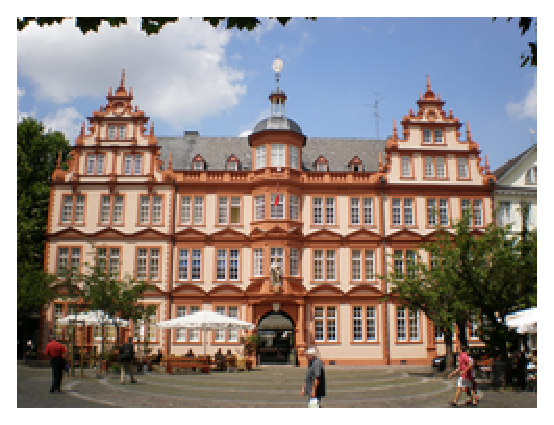
\includegraphics[height = 4 cm]{museum.eps}
  \end{figure}

  \end{frame}

\section{Dílo}

\subsection{Knihtisk}

\begin{frame}

  \frametitle{Přelomový vynález}
  
  \begin{itemize}
  
  \item Gutenberg vynalezl mechanický knihtisk na přelomu roku \textbf{1447} až \textbf{1448}.
  \item Původně pro každou tištěnou stránku musela být vytvořena zvláštní deska, což bylo značně zdlouhavé a nákladné.
  \item Gutenberg přišel s myšlenkou sestavit stranu z \textbf{písmových kuželek}, která se dala opětovně přeskupit a použít znovu, což~celý tisk podstatně zefektivnilo a~urychlilo.
  
  \end{itemize}
\end{frame}


\subsection{Znázornění}

\begin{frame}
  \begin{figure}
  	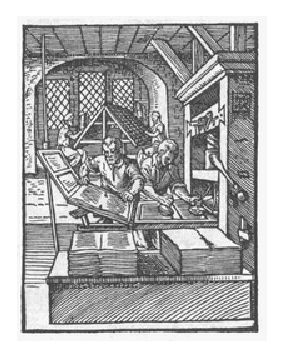
\includegraphics[height = 5 cm]{knihtisk_old.eps}
	\quad \quad
  	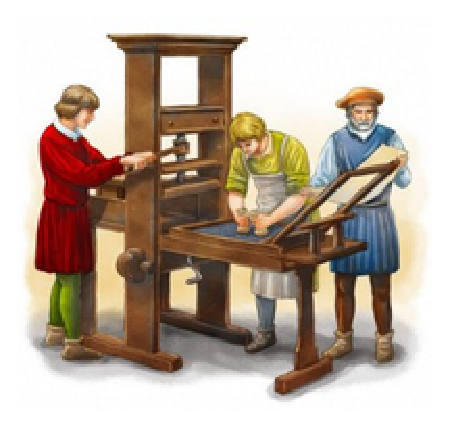
\includegraphics[height = 5 cm]{knihtisk.eps}
  \end{figure}
\end{frame}

\section{Závěr}

\subsection{Pozůstatky}

\begin{frame}
  \begin{itemize}
  \frametitle{Časová návaznost}   % Insert frame title between curly braces
  \item Následně se tisk stal \emph{reformním nástrojem} a zůstává až do dneška.
  \item Přesto, že jsou již vynalezené dokonalejší způsoby tisku jako je \textbf{ofsetový tisk}, \textbf{digitální tisk}, knihtisk neustále zůstává jedinečný k dodatečnému číslování dokumentů a tisku vizitek na lepší papír, který digitální tiskárny neumí potisknout.
  \end{itemize}
\end{frame}


\subsection{Zdroje}

\begin{frame}
  \begin{itemize}
  \frametitle{Zdroje}
  \item \url{http://knihtisk.info/index.php}
  \item \url{https://cs.wikipedia.org/wiki/Johannes_Gutenberg}
  \item \url{https://cs.wikipedia.org/wiki/Knihtisk}
  \end{itemize}
\end{frame}


\begin{frame}
  \begin{center}
		\huge{\quad Děkuji za pozornost \ldots}
  \end{center}
\end{frame}

\end{document}
